\documentclass{article}
% Paquetes adicionales
\usepackage[utf8]{inputenc} % Codificación de caracteres
\usepackage{amsmath} % Paquete para matemáticas
\usepackage{graphicx} % Para incluir gráficos
\usepackage{hyperref} % Para hipervínculos
\usepackage[spanish]{babel}
\usepackage{tabularx} % Paquete para tablas ajustables
\usepackage{float} % Paquete para la opción H en tablas y figuras
\usepackage[a4,top=2cm,bottom=2cm,left=3cm,right=3cm]{geometry}
\usepackage{algorithm} % Paquete para algoritmos
\usepackage{algpseudocode} % Paquete para pseudocódigo
\usepackage{titlesec} % Paquete para ajustar espacios de secciones
\usepackage{tabto}
\usepackage{tikz}

\titlespacing*{\subsubsection}{0pt}{\baselineskip}{0.2\baselineskip}
%Documento
\begin{document}
% Título y autores

\title{Algoritmo híbrido y evolutivo para la generación de un Ultimate Team en FIFA 19}
\author{
    20210836\\
    \textit{Piero Marcelo Pastor Pacheco}\\
    \and
    20200445\\
    \textit{Aarón Ulises Santillán Huamán}
}
\date{\today}
\maketitle
\begin{abstract}
    El siguiente trabajo tiene como objetivo implementar un algoritmo genético para la obtención de un Ultimate Team en el videojuego FIFA 2019.  El foco de esta investigación es obtener el mejor equipo que puede obtener un jugador con un presupuesto determinado, con este fin se irán minimizando factores negativos como los gastos y las edades, y maximizando otros positivos como la media en posición que jugará, potencial y química de todo el equipo en la adaptación. Para ello, se propuso una función objetivo en el cual se abarcan las variables anteriormente mencionadas y se adapta un algoritmo genético de Bin Packing para obtener un grupo de jugadores que satisfaga ser el mejor equipo. La meta es demostrar la efectividad de este algoritmo y su viabilidad en el videojuego FIFA, el cual puede ser mejorado.\newline
\end{abstract}


\section{Introdución}

Actualmente, los videojuegos se han convertido en una de las grandes industrias del mundo moderno, los cuales han evolucionado enormemente para dar al jugador una experiencia única; desde juegos de aventura hasta de deportes, estos logran transportar al usuario a experiencias inolvidables y divertidas, por lo que muchos deciden invertir su dinero en estos, según Redes Sociales (2024) “ Se trata de una industria que ha experimentado cambios significativos y que se estima que tiene unos ingresos superiores a los 180.000 millones de dólares en 2022”.  Tratándose de esta manera de una de las industrias que más mueven dinero en torno a la tecnología la cual se encuentra en un gran crecimiento.\newline
Dentro de este sector se encuentra FIFA 19, el cual es uno de los videojuegos más famosos en cuanto al fútbol,  el cual trata de implementar una experiencia inmersiva no solo en jugar un partido de fútbol, sino también en el manejo de un equipo, teniendo un presupuesto con el cual se puede contratar jugadores y obtener la victoria, obteniendo de esta manera una experiencia más inmersiva al mundo del fútbol. De modo que nace la pregunta ¿Cómo puede un algoritmo genético permitir obtener los mejores jugadores para un Ultimate Team en el videojuego FIFA 2019?\newline
Normalmente para la elaboración de un equipo para algún deporte, existe siempre la limitante del presupuesto. El algoritmo que se presentará a continuación trata de bajo un presupuesto por más mínimo que sea, conseguir generar un buen equipo de fútbol. Esto se llevará a cabo maximizando la media en las posiciones de jugadores, potencial de juego, y química; mientras que se buscará minimizar el precio para siempre ahorrar lo mayor posible, y la edad de los jugadores teniendo preferencia por los más jóvenes.\newline
Además de solucionar este problema, se buscará comparar un algoritmo híbrido que sea la combinación de un genético evolutivo y un GRASP (Greedy Randomized Adaptive Search Procedure), con un algoritmo genético evolutivo puro.\newline
Los resultados nos ofrecerán una comparación para saber si vale la pena el costo computacional extra de un GRASP dentro de un evolutivo, o si la diferencia de resultados es mínima y no es necesario; considerándose así un desperdicio la implementación del híbrido.

\section{Trabajos relacionados}
\subsection{Heurísticas de agrupación híbridas eficientes para el problema de empacado de objetos en contenedores }
El artículo aborda el clásico problema de empaquetado (Bin Packing Problem), pero mediante un enfoque del uso de un algoritmo genético híbrido de agrupación denominado HGGA-BP, el cual está inspirado en el esquema de representación de grupos de Falkenauer.\newline
En el caso de este artículo, se tiene la restricción del peso de cada uno de los contenedores empleados para guardar paquetes de determinado peso, en nuestro caso, se tendrá el presupuesto (peso de dinero no podemos sobrepasar al igual que los contenedores. \newline
Asimismo, emplea el siguiente pseudocódigo en la implementación:\newline
\begin{figure}[H]
    \centering
    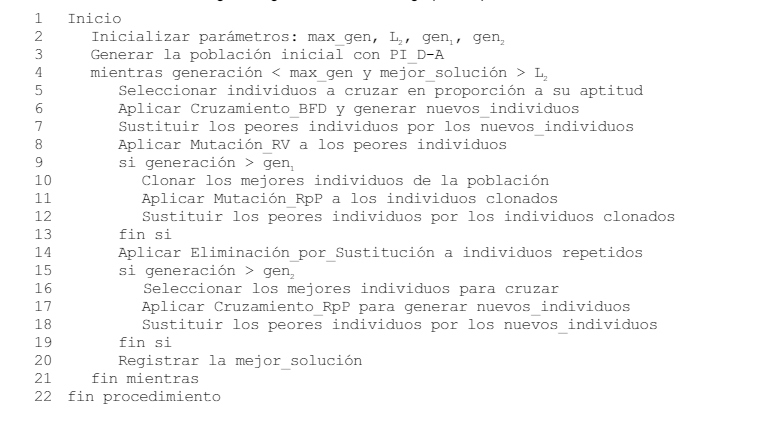
\includegraphics[width=1\linewidth]{imagenes/image1.png}
    \caption{Algoritmo genético híbrido de agrupación para BPP: HGGA-BP.}
    \label{fig:enter-label}
\end{figure}
En esta imagen, se puede visualizar el algoritmo empleado para el artículo como también las operaciones genéticas para grupos como el cruzamiento, mutación y eliminación, los cuales son de gran utilidad al obtener las mejores soluciones.\newline
La conclusiones de este trabajo es que el tiempo de ejecución del algoritmo propuesto es muy corto, la cual presenta una calidad de soluciones similar a los algoritmos del estado del arte.

\subsection{Implementación de un algoritmo memético para optimizar la carga de hornos para la producción de sanitarios}
El presente trabajo tiene como objetivo la implementación de un algoritmo memético para optimizar la carga de hornos de cerámicos frente a la continua competencia entre las empresas de este sector.  En este se plantea la comparación entre este algoritmo y uno genético para el problema de la selección de piezas en la producción de sanitarios, el cual tiene restricciones como el peso máximo de las vagonetas, volumen máximo del horno, etc. \newline
Para este, se plantea el siguiente pseudocódigo: \newline
\begin{figure}[H]
    \centering
    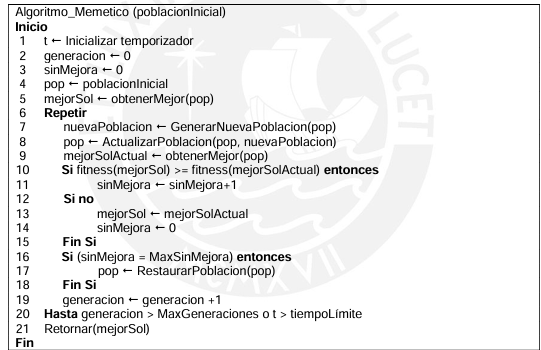
\includegraphics[width=1\linewidth]{imagenes/image4.png}
    \caption{Pseudocódigo del algoritmo memético.}
    \label{fig:enter-label}
\end{figure}
Este trabajo plantea la generación de una población inicial usando el algoritmo GRASP, el cual aportará en gran medida al algoritmo memético en la obtención del mejor resultado, en el cual al ser calibrado se obtiene un alpha de valor 0.4.
Las conclusiones que este trabajo presenta, es que el algoritmo memético logra dar mejores soluciones que el algoritmo genético, no obstante, no es lo suficientemente significativa, por lo que se considera que ambas logran dar soluciones igualmente buenas.

\subsection{A distributed Chromosome genetic algorithm for bin-packing}
Este trabajo plantea a los algoritmos genéticos como un enfoque muy bueno en la resolución de problemas de optimización, en el cual se detalla el desarrollo de un cromosoma GA distribuido para reducir el tiempo de ejecución del GARP el cual tiene como fin el resolver el problema de empaquetamiento de cilindros de construcción creados por la Universidad de Louisville en contenedores de Sinterstation 2000.
Para esto, se utilizan algoritmos genéticos distribuidos con el fin de reducir el tiempo de ejecución, para ello, se tiene en cuenta la sobrecarga de comunicación así como la sincronización. 
Se debe de tener conocimiento, que el empaquetado se realiza en contenedores tridimensionales, en el cual el algoritmo requiere un uso computacional intensivo y más cuando se trata de objetos definidos por archivos de modelo sólido o estereolitografía, para lo cual utilizan un gran cantidad de parámetros al ser analizadas.
En la conclusión demuestran que el uso de un cromosoma GA distribuido disminuye el tiempo de ejecución, no obstante los resultados obtenidos del algoritmo son buenos, aún así, los autores plantean que una mejora se haría mediante una configuración del hardware.


\section{Metodología}
\subsection{Descripción del problema}
El artículo busca solucionar el problema de la generación de equipos de fútbol, pero al mismo tiempo busca realizar un análisis a los resultados de dos tipos de algoritmos metaheurísticos.\newline
El algoritmo híbrido buscará mejorar mediante la selección, la media y química del equipo; minimizando gastos para que así el usuario pueda seleccionar más adelante a un jugador de élite de su gusto (en caso el algoritmo no lo haya colocado ya en su equipo). El GRASP se verá reflejado en la generación de una población inicial, que si bien puede ser randonomica, esta siempre buscará maximizar el fitness tanto del jugador individual como del equipo general. El resto del algoritmo evolutivo mantiene los estándares comunes, implementando una función que elimina las aberraciones, otra que se encarga de los clones, y una última que con cada generación limita la población disminuyéndola en un porcentaje; si bien esta última selección es randonomica, siempre da preferencia a eliminar a la población con peor fitness. \newline
El algoritmo evolutivo puro, trabaja de la misma manera que el híbrido en el ámbito que corresponde a un algoritmo genético. La única diferencia es la forma en que se genera la población inicial, este algoritmo la genera randonomicamente, solo tiene como restricción el no crear aberraciones.

\subsection{Entrada y Salida}
Ambos algoritmos recibirán un grupo de jugadores del juego, aquí se encontrará por jugador los siguientes valores:

\begin{table}[H]
    \centering
    \begin{tabularx}{\columnwidth}{|X|X|X|}
        \hline
        Atributo & Tipo de dato & Descripción \\
        \hline
        id & Integer & ID del jugador\\
        nombre & String & Nombre del jugador \\
        nacionalidad & String & Nacionalidad del jugador\\
        posicion & String & Posición principal del jugador\\
        media & Integer & Media general del jugador\\
        potencial & Integer & Potencial de juego del jugador\\
        club & String & Club del jugador\\
        valor & Double & Valor en M€\\
        mediasPos & Map<String, Integer> & Media de juego en cada posición del campo\\
        
        \hline
    \end{tabularx}
    \caption{Atributos de un jugador.}
    \label{tab:etiqueta}
\end{table}

Se utilizaron varias posiciones, para que si una posición ya está tomada, pero si este jugador se desenvuelve igual de bien en otra; pueda ser enviado a esa.\newline
La entrada por parte del usuario es únicamente que formación se utilizará y que presupuesto es el que posee para poder armar su equipo.\newline
La salida es el equipo formado en cada posición y el fitness que generó este individuo en la población.

\subsection{Constantes}
Las constantes seleccionadas se consiguieron tras una calibración que evaluaba el fitness promedio entre ejecuciones. Este proceso se explicará a mayor detalle en la parte de \hyperref[sec:exp]{experimentación}. Es importante hacer inciso en que las únicas constantes que han sido calibradas son las que corresponden a porcentajes de la data; tanto $POBINICIAL$, como $GENERACIONES$ no han sido calibrados, ya que, únicamente son valores de inicio o topes.
\subsubsection{Metaheurístico Híbrido}
Las constantes utilizadas para maximizar el fitness en el algoritmo híbrido entre evolutivo y GRASP son: \newline
\begin{table}[H]
    \centering
    \begin{tabularx}{\columnwidth}{|l|c|X|}
        \hline
        Constante & Valor & Descripción \\
        \hline
        Tcasamiento & 0.7 & Que porcentaje de la población serán padres\\
        Tmutacion & 0.0 & Que porcentaje de los padres mutarán \\
        Tmuerte & 0.1 & Que porcentaje de la población se eliminará\\
        Pcasamiento & 0.4 & Que porcentaje le corresponderá del padre al nuevo cromosoma\\
        POBINICIAL & 50 & De que tamaño será la población que se generará\\
        GENERACIONES & 100 & Cantidad de generaciones máximas que realizará el algoritmo \\
        ALPHA & 0.3 & Porcentaje que se tomará para optimizar los resultados del GRASP\\
        \hline
    \end{tabularx}
    \caption{Constantes del híbrido}
    \label{tab:etiqueta}
\end{table}

\subsubsection{Genético Evolutivo}
Las constantes utilizadas para maximizar el fitness en el algoritmo evolutivo puro son: \newline
\begin{table}[H]
    \centering
    \begin{tabularx}{\columnwidth}{|l|c|X|}
        \hline
        Constante & Valor & Descripción \\
        \hline
        Tcasamiento & 0.7 & Que porcentaje de la población serán padres\\
        Tmutacion & 0.0 & Que porcentaje de los padres mutarán \\
        Tmuerte & 0.1 & Que porcentaje de la población se eliminará\\
        Pcasamiento & 0.8 & Que porcentaje le corresponderá del padre al nuevo cromosoma\\
        POBINICIAL & 50 & De que tamaño será la población que se generará\\
        GENERACIONES & 100 & Cantidad de generaciones máximas que realizará el algoritmo \\
        \hline
    \end{tabularx}
    \caption{Constantes del evolutivo puro}
    \label{tab:etiqueta}
\end{table}

\subsection{Algoritmos empleados}

A continuación se tendrán los pseudocódigos de cada función que tenga alta relevancia empleada para los algoritmo, además de la programación metódica que demostrará el correcto funcionamiento del fitness.

\subsubsection{Metaheurístico Híbrido}

\floatname{algorithm}{Metaheurístico Híbrido}
\renewcommand{\thealgorithm}{}
\begin{algorithm}[H]
    \caption{Algoritmo para encontrar el mejor equipo en el videojuego FIFA 19} 
    \begin{algorithmic}[1]
        \Procedure{hibrido}{$jugadores, n, presupuesto, posiciones, quimica$} \Comment{Halla el mejor equipo en base al presupuesto}
            \State \Call{GRASP}{$jugadores, poblacion, n, presupuesto, posiciones, quimica, POBINICIAL$}
            \State $i \gets 0$
            \While{$i \neq GENERACIONES \land tampoblacion > 1 $}
                \State \Call{Seleccion}{$poblacion, padres, jugadores, n, posiciones, quimica$}
                \State \Call{Casamiento}{$poblacion, padres$}
                \State \Call{Mutacion}{$poblacion, padres, jugadores$}
                \State \Call{EliminarAberraciones}{$poblacion, jugadores, presupuesto$}
                \State \Call{EliminarClones}{$poblacion$}
                \State \Call{DisminuirPoblacion}{$poblacion, jugadores, n, posiciones, quimica$}
                \State $i = i+1$
            \EndWhile
            \State \Call{Seleccion}{$poblacion, padres, jugadores, n, posiciones, quimica$}
            \State \textbf{return } \Call{Random}{$padres$} \Comment{Retorna el mejor equipo}
        \EndProcedure
    \end{algorithmic}
\end{algorithm}

\floatname{algorithm}{FitnessIndividuo}
\renewcommand{\thealgorithm}{}
\begin{algorithm}[H]
    \caption{Algoritmo para encontrar el mejor equipo en el videojuego FIFA 19} 
    \begin{algorithmic}[1]
        \Procedure{FitnessIndividuo}{$equipo, posiciones, quimica$} \Comment{Halla el fitness de todo el equipo}
            \State $fo\_max \gets \Call{Media}{equipo[0]} * \Call{Potencial}{equipo[0]}$
            \State $fo\_min \gets \Call{Valor}{equipo[0]} * \Call{Edad}{equipo[0]}$
            \State $i \gets 1$
            \While{$i < N\_PLAYERS$}
                \State $fo\_max \gets fo\_max + \Call{MediaPosicion}{equipo[i]} * \Call{Potencial}{equipo[i]}$
                \State $fo\_min \gets fo\_min + \Call{Valor}{equipo[i]} * \Call{Edad}{equipo[i]}$
                \State $i = i+1$
            \EndWhile
            \State $i \gets 0$
            \State $QuimParcial \gets 0$
            \While{$i < N\_CHEM$}
                \State $j \gets 0$
                \While{$j < N\_CHEM$}
                    \If{$quimica[i][j] \neq -1 $}
                        \State $index \gets quimica[i][j]$
                        \State $Cant\_Relaciones \gets Cant\_Relaciones + 1$
                            \If{$\Call{Nacionalidad}{equipo[i]} = \Call{Nacionalidad}{equipo[index]} \land \Call{Club}{equipo[i]} = \Call{Club}{equipo[index]}$}
                                \State $QuimParcial \gets QuimParcial + 200$
                            \Else 
                                \If{$\Call{Nacionalidad}{equipo[i]} = \Call{Nacionalidad}{equipo[index]} \lor \Call{Club}{equipo[i]} = \Call{Club}{equipo[index]}$}
                                    \State $QuimParcial \gets QuimParcial + 100$
                                \Else
                                    \State $QuimParcial \gets QuimParcial + 60$
                            \EndIf
                        \EndIf
                    \Else
                    \State \textbf{break }
                    \EndIf
                    \State $j = j+1$
                \EndWhile
                \State $i = i+1$
            \EndWhile
            \State $QuimParcial \gets QuimParcial \div (Cant\_Relaciones \times 100)$
            \If{$QuimParcial > 1$}
            \State $QuimParcial \gets 1$
            \EndIf
            \State \textbf{return }{$(fo\_max \times QuimParcial) \div (fo\_min \times PER\_MIN)$}
        \EndProcedure
    \end{algorithmic}
\end{algorithm}

\subsubsection{GRASP}

\floatname{algorithm}{Metaheurístico GRASP}
\renewcommand{\thealgorithm}{}
\begin{algorithm}[H]
    \caption{Algoritmo para elaborar la población inicial del híbrido}
    \begin{algorithmic}[1]
        \Procedure{GRASP}{$jugadores, poblacion, n, presupuesto, posiciones, quimica, requerido$} \Comment{Halla una población inicial aceptable}
            \State $i \gets 0$
            \While{$i \neq ITERACIONES$}
                \State $foparcial \gets$ \Call{Construccion}{$mediasPosicion, pobParcial, n, presupuesto, posiciones, quimica$}
                \State $foparcial \gets foparcial * $ \Call{HallarQuimica}{$pobParcial, jugadores, quimica$} \Comment{Halla la química de todo el equipo, ya que, la construcción no puede hacerlo por si sola}
                \State \Call{ActualizarMejores}{$poblacion, pobParcial, mejoresFo, foParcial, requerido$} \Comment{Actualiza la población inicial con el nuevo individuo conseguido}
                \State $i \gets i + 1$
            \EndWhile
        \EndProcedure
    \end{algorithmic}
\end{algorithm}

\floatname{algorithm}{Metaheurístico GRASP}
\renewcommand{\thealgorithm}{}
\begin{algorithm}[H]
    \small
    \caption{Construcción de la población inicial}
    \begin{algorithmic}[1]
        \Procedure{Construccion}{MediaDePosicion, candidato, n, presupuesto, posiciones, chem\_pos}
            \State $fitness \gets 0$
            \State $borrados \gets$ lista vacía
            
            \Comment{Análisis exclusivo de arqueros}
            \While{true}
                \State $beta \gets Mejor(MediaDePosicion["GK"])$
                \State $tau \gets 0$
                \State $maxrcl \gets beta - ALPHA \times (beta - tau)$
                \State $indmax \gets beta - maxrcl$
                \State $inda \gets$ (si $indmax > 0$) ? aleatorio \% $indmax$ : $0$
                \State $inda \gets inda + maxrcl$
                \State $JugadorActual \gets MediaDePosicion[posiciones[0]]$
                \If{$presupuesto \geq \Call{Valor}{JugadorActual}$}
                    \State $presupuesto \gets presupuesto - \Call{Valor}{JugadorActual}$
                    \State $candidato[0] \gets JugadorActual$
                    \State $fitness \gets fitness + \Call{Fitness}{JugadorActual}$
                    \State \textbf{break}
                \EndIf
            \EndWhile
            \State
            \For{$i \gets 1$ to $N\_PLAYERS - 1$}
                \State $beta \gets Mejor(MediaDePosicion[Posiciones[i]])$
                \State $tau \gets 0$
                \State $maxrcl \gets beta - ALPHA \times (beta - tau)$
                \State $indmax \gets beta - maxrcl$
                \State $inda \gets$ (si $indmax > 0$) ? aleatorio \% $indmax$ : $0$
                \State $inda \gets inda + maxrcl$
                \State $JugadorActual \gets MediaDePosicion[posiciones[i]]$
                \If{$presupuesto \geq \Call{Valor}{JugadorActual} \land 
                    Posicion(MediaDePosicion[Posiciones[i]]) \neq "GK"$}
                    \State $presupuesto \gets presupuesto - \Call{Valor}{JugadorActual}$
                    \State $candidato[i] \gets JugadorActual$

                    \State $fitness \gets fitness + \Call{Fitness}{JugadorActual}$
                \Else
                    \State $i \gets i - 1$ \Comment{Tiene que volver a analizar la posición}
                \EndIf
                \State \Call{Borrar}{$JugadorSeleccionado$}
            \EndFor
            \State \Return $fitness$
        \EndProcedure
    \end{algorithmic}
\end{algorithm}

\subsubsection{Genético Evolutivo}

\begin{algorithm}[H]
    \caption{Algoritmo para encontrar el mejor equipo en el videojuego FIFA 19} 
    \begin{algorithmic}[1]
        \Procedure{hibrido}{$jugadores, n, presupuesto, posiciones, quimica$} \Comment{Halla el mejor equipo en base al presupuesto}
            \State \Call{GenerarPoblacion}{$jugadores, poblacion, n, presupuesto, posiciones, quimica, POBINICIAL$}
            \State $i \gets 0$
            \While{$i \neq GENERACIONES \land tampoblacion > 1 $}
                \State \Call{Seleccion}{$poblacion, padres, jugadores, n, posiciones, quimica$}
                \State \Call{Casamiento}{$poblacion, padres$}
                \State \Call{Mutacion}{$poblacion, padres, jugadores$}
                \State \Call{EliminarAberraciones}{$poblacion, jugadores, presupuesto$}
                \State \Call{EliminarClones}{$poblacion$}
                \State \Call{DisminuirPoblacion}{$poblacion, jugadores, n, posiciones, quimica$}
                \State $i \gets i+1$
            \EndWhile
            \State \Call{Seleccion}{$poblacion, padres, jugadores, n, posiciones, quimica$}
            \State \textbf{return } \Call{Random}{$padres$} \Comment{Retorna el mejor equipo}
        \EndProcedure
    \end{algorithmic}
\end{algorithm}

\subsubsection{Programación Metódica Fitness}

\State \textbf{G}{$: (\boldsymbol{\forall} \ i : 1 \leq i < n : Posicion(equipo[i]) \neq "GK" )$}
\State $\{Pre: N = 11 \land equipo \neq \emptyset \ \land \ posiciones \neq \emptyset \ \land \ quimica \neq \emptyset \ \land \ Posicion(equipo[0]) = "GK" \land \ \textbf{G} \}$ 
\State \textbf{proc }{$HallarFitness(\textbf{value} \ equipo : \textbf{array \ of}\ Equipo;$}
\State \tabto{63} $\textbf{value} \ posiciones : \textbf{array \ of} \ string; $
\State \tabto{63} $\textbf{value} \ quimica : \textbf{array \ of}\ \textbf{array \ of} \ integer);$
\State \tabto{63} $\textbf{result} \ fitness : double);$
\State \tabto{25} $fo\_max := Media(equipo[0]) \times Potencial(equipo[0])$
\State \tabto{25} $fo\_min := Valor(equipo[0]) \times Edad(equipo[0])$
\State \tabto{25} $i := 0$
\State \tabto{25} $\{invariant: fo\_max > 0 \land fo\_min > 0\}$
\State \tabto{25} $\{bound: N-1\}$
\State \tabto{25} $\textbf{do}\ i < N \rightarrow fo\_max := fo\_max + Media(equipo[i]) \times Potencial(equipo[i]), fo\_min := fo\_min +$
\State \tabto{81} $Valor(equipo[i]) \times Edad(equipo[i]), i := i + 1 \  $
\State \tabto{25} $\textbf{od}$
\State \tabto{25} $i, QuimParc, Cant\_Relaciones := 0$
\State \tabto{25} $\{invariant: 0 \leq QuimicaParc\}$
\State \tabto{25} $\{bound: N-2\}$
\State \tabto{25} $\textbf{do}\ i < N-1 \rightarrow j := 0, $
\State \tabto{75} $\{bound: N-2\}$
\State \tabto{75} $\textbf{do}\ j < N-1 \rightarrow$
\State \tabto{127} $\textbf{if}\ quimica[i][j] \neq -1 \rightarrow index := quimica[i][j], Cant\_Relaciones := $
\State \tabto{232} $Cant\_Relaciones + 1, $
\State \tabto{204} $\textbf{if}\ Nacionalidad(equipo[i]) = Nacionalidad(equipo[index]) \ \land $
\State \tabto{214} $Club(equipo[i]) = Club(equipo[index])\rightarrow QuimParc := $
\State \tabto{214} $QuimParc +200$
\State \tabto{207.5} $\tikz \draw (0,0) rectangle (0.1,0.25); \ Nacionalidad(equipo[i]) = Nacionalidad(equipo[index]) \ \lor $
\State \tabto{214} $Club(equipo[i]) = Club(equipo[index])\rightarrow QuimParc := $
\State \tabto{214} $QuimParc +100$
\State \tabto{207.5} $\tikz \draw (0,0) rectangle (0.1,0.25); \ \textbf{True} \ \rightarrow QuimParc := QuimParc +65$
\State \tabto{204} $\textbf{fi}$
\State \tabto{133.5} $\tikz \draw (0,0) rectangle (0.1,0.25); \ quimica[i][j] = -1 \ \rightarrow j := N-1$
\State \tabto{127} $\textbf{fi}, \ j := j + 1$
\State \tabto{77} $\textbf{od}, \ i := i + 1$
\State \tabto{25} $\textbf{od}$
\State \tabto{25} $\{postcondition: 65 \leq QuimicaParc\}$
\State \tabto{25} $QuimicaParc := QuimicaParc \div (Cant\_Relaciones \times 100)$
\State \tabto{25} $\textbf{if} \ QuimcaParc > 1 \rightarrow QuimParc := 1 \ \textbf{fi}$
\State \tabto{25} $fitness := (fo\_max \times QuimicaParc) \div (fo\_min \times PER\_MIN)$
\State $\{Post: fitness > 0\}$
\State
\State Otra forma de entenderlo es:
\State \textbf{G}{$: (\boldsymbol{\forall} \ i : 1 \leq i < n : Posicion(equipo[i]) \neq "GK" )$}
\State \textbf{Q}{$: \{N = 11 \land equipo \neq \emptyset \ \land \ posiciones \neq \emptyset \ \land \ quimica \neq \emptyset \ \land \ Posicion(equipo[0]) = "GK" \land \ \textbf{G} \}$}
\State \textbf{R}{$: \{fitness > 0\}$}

\State $\textbf{Q} \implies wp(HallarFitness, \textbf{R})$

\section{Experimentación y Resultados}
\label{sec:exp}
\subsection{Calibración}

Para la calibración de constantes se utilizaron varias ejecuciones las cuales se fueron almacenando en archivos ".csv". Y de esta forma poder tener almacenado el histórico de cada valor que se cambiaba para tener un máximo preciso. Dichos archivos se encuentran en el repositorio del proyecto.

\subsection{Comparación}
Para la evaluación de los algoritmos y conocer tanto sus resultados independientes, como una comparación que nos pueda indicar que proceso es el que proporciona mejores resultados; se realizará una ejecución con la cual podamos tener 100 fitness resultado de cada uno de los algoritmos para posteriormente tener gráficas estadísticas y así poder sacar conclusiones. Estas gráficas se consiguieron utilizando el lenguaje de programación Python.

\subsubsection{Gráfico de Dispersión}

Se utilizó este gráfico para poder conocer a simple vista utilizando puntos el algoritmo que tiende a dar mejores resultados con más frecuencias, incluyendo los picos de cada uno.
\begin{figure}[H]
    \centering
    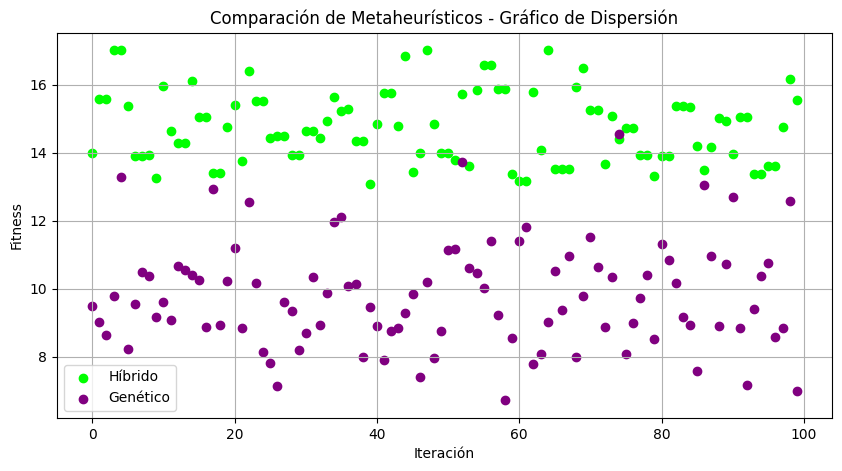
\includegraphics[width=1\linewidth]{imagenes/grafico_dispersion.png}
    \caption{Gráfico de dispersión - Autoría propia}
    \label{fig:enter-label}
\end{figure}

\subsubsection{Gráfico Lineal}

El gráfico lineal resultó útil para unir todos los puntos del gráfico de dispersión y poder conocer como eran las variaciones del fitness entre ejecuciones.

\begin{figure}[H]
    \centering
    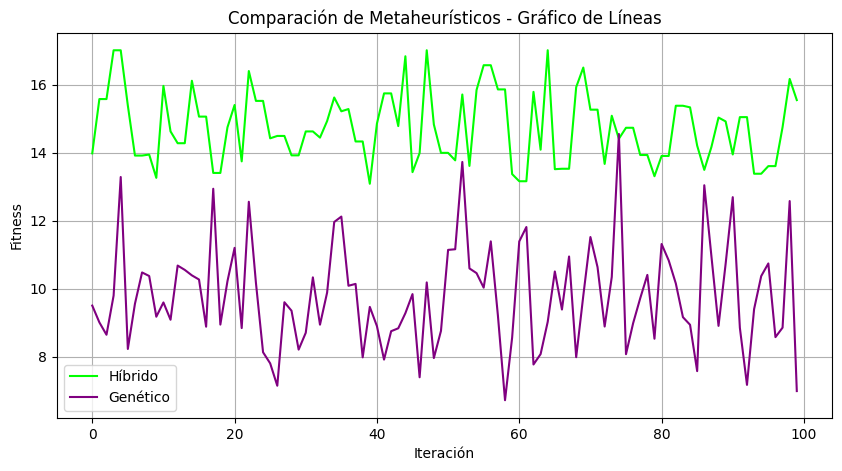
\includegraphics[width=1\linewidth]{imagenes/grafico_lineal.png}
    \caption{Gráfico lineal - Autoría propia}
    \label{fig:enter-label}
\end{figure}

\subsubsection{Gráfico BoxPlot}

Con este gráfico podemos analizar los percentiles más importantes de los resultados, así como saber que datos atípicos existen por parte de cada algoritmo.

\begin{figure}[H]
    \centering
    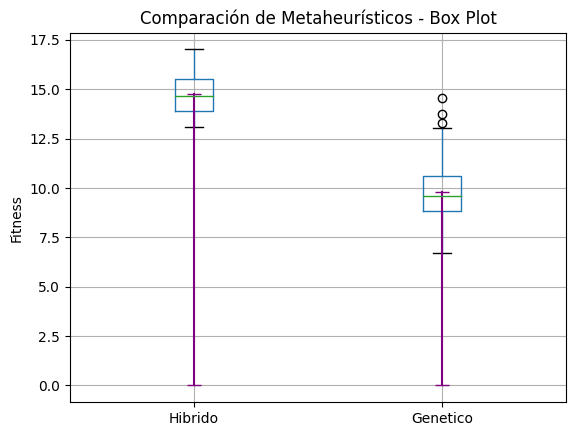
\includegraphics[width=0.75\linewidth]{imagenes/grafico_boxplot.png}
    \caption{Gráfico BoxPlot - Autoría propia}
    \label{fig:enter-label}
\end{figure}

\subsubsection{Gráfico Histograma}

Este cuarto gráfico es útil para saber un promedio aproximado del resultado que consiguieron cada una de las iteraciones, además de que tan probable es que consigan datos muy altos (atípicos). \newline
Este último análisis es el más importante junto con el BoxPlot porque nos permiten de manera más directa analizar los promedios y que porcentaje es la probabilidad que se consigan resultados excelentes. Además de poder analizar en que algoritmo los resultados son muy variados, es decir, que pueden dispararse tanto como para resultados esperados, como a los peores.

\begin{figure}[H]
    \centering
    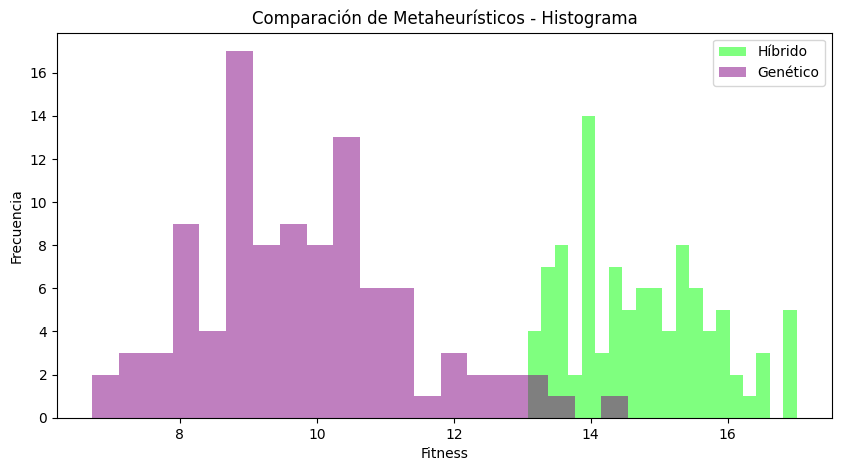
\includegraphics[width=1\linewidth]{imagenes/grafico_histograma.png}
    \caption{Gráfico Histograma - Autoría propia}
    \label{fig:enter-label}
\end{figure}

\section{Conclusión}

De acuerdo con lo señalado y los resultados mostrados, se puede concluir principalmente que ambos algoritmos logran dar una respuesta ante la generación de un Ultimate Team para un jugador que cuenta con un presupuesto determinado. No obstante, según las gráficas se puede visualizar que mediante el algoritmo meta heurístico híbrido se logra obtener mejores resultados, ya que los resultados en 100 iteraciones suelen rondar entre los 13 y 17 de fitness promedio, mientras que el algoritmo genético evolutivo suele originar fitness entre 7 y 13, y aunque en pocas ocasiones se logra obtener fitness de 14, estos son valores atípicos.\newline
En la prueba de calibraciones de las tasas para ambos algoritmos se pudo observar que es también el algoritmo meta heurístico híbrido el que logra dar un resultado en el menor tiempo, ya que el tiempo promedio de salida rondaba en 1 minuto con 30 segundos. Por otro lado, el algoritmo genético evolutivo daba una respuesta promedia de 10 minutos, llegando incluso a 1 hora con ciertas tasas.\newline
Esto puede estar estrechamente relacionado con cómo está construido el algoritmo, ya que para ambos algoritmos hay una fase de eliminación de aberraciones al generar población, y el híbrido al utilizar GRASP suele tener poblaciones que no requieran tomar el proceso de eliminación ya que no son aberradas. Por otro lado, el algoritmo genético evolutivo al generar poblaciones aleatorias suele tener un mayor uso de esta función, incrementando así el uso de esta función tanto en la generación de poblaciones como en las posteriores funciones como el eliminado por menor fitness y una última eliminación de aberraciones.\newline
De este modo, se puede concluir que el uso de un algoritmo meta heurístico híbrido logra emitir mejores y más rápidos resultados en cuanto a la generación del Ultimate Team de FIFA 19, los cuales pueden ayudar al jugador en cuanto a la decisión de generación de equipos al momento de jugar.

\section{Sugerencia de trabajos futuros}

Principalmente, una sugerencia debería ser tener un periodo de calibración de constantes más extenso, ya que aunque las tasas tanto de casamiento, mutación, eliminación y probabilidad de casamiento duraron 15 horas en ser calibradas, se puede mejorar la precisión en estas constantes si el periodo fuera más extenso.
Asimismo, mediante estas calibraciones se encontró que la mejor tasa de mutación es de 0. Lo cual para futuros trabajos puede ser eliminado de las funciones ya que posiblemente la mutación al ser aleatoria esté generando peores resultados.\newline
Otra sugerencia a tomar está en cuanto a los datos, este trabajo fue realizado para FIFA 19, un juego que ya lleva varios años desde su lanzamiento, en el cual ya hay múltiples juegos más actuales, se puede sugerir tomar los datos más actuales ya que estos pueden ser de mayor beneficio ya que es donde se encuentra actualmente la comunidad.\newline
Por último, este trabajo tomó en cuenta un "alpha" de 0.4 para la implementación del GRASP, esto debido al trabajo relacionado “Implementación de un algoritmo memético para optimizar la carga de hornos para la producción de productos sanitarios”. No obstante, esta constante es un valor que debe ser calibrado para futuros trabajos.


\section{Implicancias éticas}

Las implicaciones éticas giran en torno a la forma en cómo se desarrolla el juego en la actualidad. En la que se contempla tres factores principales: \newline

\subsection{Equidad y Competitividad}
    Si se comparte o vende el algoritmo, esto podría afectar seriamente a las partidas en línea con las que cuenta FIFA 19, en las que algunos jugadores pueden considerar injusto el uso de un algoritmo para obtener el Ultimate Team  ya que el juego actualmente se basa en la experiencia manual. Esto podría solucionarse al no dar directamente el algoritmo a la comunidad sino a la empresa del juego “EA Sports”, los cuales pueden implementarlo como una función dentro del juego para que cualquier jugador pueda utilizarlo si lo desea.

\subsection{Economía}

    Esto ya que el algoritmo al encontrar a los mejores jugadores podrían solo concentrarse en comprar y vender jugadores en específico, desequilibrando el mercado dentro del juego. Esto se podría solucionar al afectar un poco el algoritmo para que logre emitir una solución promedio, que no siempre sea la mejor pero tampoco la peor, dando al jugador la perspectiva de que es una máquina de sugerencia, más para la decisión de formar el Ultimate Team es el criterio propio.

\subsection{Transparencia}

    Si se comparte o vende el algoritmo, se debe ser transparente con los jugadores y la empresa de cómo realmente funciona, ya que algunos jugadores podrían tomarlo como si fuera trampa, y si la empresa determina que efectivamente es trampa podría llegar a convertirse en un software ilegal, lo cual podría escalar a términos legales. Por ello, siempre se debe ser transparente y honesto en cuanto a cómo funcionan los algoritmos.

\section{Repositorio de GitHub}

\href{https://github.com/PieroPastor/Algoritmo-hibrido-y-evolutivo-para-la-generacion-de-un-Ultimate-Team-en-FIFA-19.git}{Repositorio - Algoritmo híbrido y evolutivo para la generación de un Ultimate Team en FIFA 19}

\section{Declaración de contribución de cada integrante}
\subsection{Aporte de Alumno Santillán Huamán, Aarón Ulises - 20200445}
Realizó la introducción del informe, así como sintetizar los trabajos relacionados para obtener tasas y constantes iniciales para la calibración de los algoritmos.\newline
Además, se encargó de la búsqueda y calibración de las constantes de tasa y probabilidad utilizadas en los algoritmos. Asimismo, realizó las diapositivas para la exposición en aula.\newline
Por último, redactó las conclusiones del informe e Implicancias éticas de este. 
\subsection{Aporte de Alumno Pastor Pacheco, Piero Marcelo - 20210836}
Realizó los algoritmos, además de sus respectivos pseudocódigos y la programación metódica para el fitness.\newline
De igual manera realizó la experimentación y comparación entre ambos algoritmos, esto utilizando gráficas estadísticas.\newline
Por último redactó el reporte en Latex.

\section{Referencias}

Cruz-Reyes, L., C, M. Q., Alvim, A. C. F., Huacuja, H. J. F., S, C. G., & Torres-Jiménez, J. (2012). Heurísticas de agrupación híbridas eficientes para el problema de empacado de objetos en contenedores. Redalyc.org. https://www.redalyc.org/articulo.oa?id=61524403009\newline

Bankinter. (12 de enero de 2024). Estudio mercado videojuegos: ¿Cuánto dinero mueve? (infografía). Bankinter. https://www.bankinter.com/blog/finanzas-personales/mercado-videojuegos-dinero-estudio-espana-mundo\newline

Malgrejo P. & Melgarejo N. (2019, 28 octubre). Implementación de un algoritmo memético para optimizar la carga de hornos para la producción de sanitarios. http://hdl.handle.net/20.500.12404/15273\newline

Lewis, J. E., Ragade, R. K., Kumar, A., & Biles, W. E. (2005). A distributed chromosome genetic algorithm for bin-packing. Robotics And Computer-integrated Manufacturing, 21(4-5), 486-495. https://doi.org/10.1016/j.rcim.2004.11.017



\end{document}